 \documentclass[a4paper,12pt]{report}
\usepackage[spanish,mexico]{babel}
\usepackage[utf8]{inputenc}
\usepackage[T1]{fontenc}
\usepackage{amsmath}
\usepackage{amssymb}
\usepackage{wasysym}
\usepackage[dvipsnames,pdftex]{color}
\usepackage[x11names]{xcolor}
\usepackage{tikz, tkz-euclide}
\usepackage[american]{circuitikz}
\usepackage{siunitx}
\usetikzlibrary{arrows}
\usepackage[colorinlistoftodos]{todonotes}
%\usepackage[left=2cm,right=1.5cm,top=1cm,bottom=1cm]{geometry}
%\usepackage{helvet}
%\renewcommand{\familydefault}{\sfdefault}
\setlength{\oddsidemargin}{0in}
\usepackage{geometry}
\geometry{a4paper, total = {180mm,270mm},
			left = 25mm, top = 20mm,
            right=15mm,bottom=20mm,%
            footskip=10mm}
\usepackage{float} 
% \setlength{\topmargin}{0in}
% \setlength{\voffset}{-0.5in}
% \setlength{\hoffset}{0.3in}
% \setlength{\textheight}{700pt}
% \setlength{\textwidth}{440pt}
% \setlength{\topskip}{0in}
% \setlength{\parskip}{2ex}
 \renewcommand{\baselinestretch}{1.5}
\usepackage{diagbox}
\usepackage{array}
\usepackage{listings}
\usepackage{caption}
%%% comandos definidos por el usuario
\begin{document}
\setcounter{page}{1}
\pagenumbering{roman}
\thispagestyle{empty}
\begin{center}
{\huge UNIVERSIDAD NACIONAL DE INGENIERÍA}\\[0.9cm]
{\Large FACULTAD DE INGENIERÍA MECÁNICA}\\[0.6in]
\end{center}
\begin{figure}[h]
\begin{center}

\includegraphics[scale=0.33]{logoUNI.png}
\vspace{0cm}
\end{center}
\end{figure}
\vspace{0.5cm}
\begin{center}
INFORME DE LABORATORIO\\
LABORATORIO DE CIRCUITOS ELÉCTRICOS\\[5mm]
{\large RELACIONES ESCALARES Y COMPLEJAS EN CIRCUITOS ELÉCTRICOS LINEALES AC}\\[10mm]
\vfill
LIMA - PERÚ \hfill NOVIEMBRE 2019
\end{center}
\newpage
\thispagestyle{empty}
\begin{center}
{\Huge RELACIONES ESCALARES Y COMPLEJAS EN CIRCUITOS ELÉCTRICOS LINEALES AC}\\[0.7cm]
\small ENTREGADO:\\[0.05cm]
\small 06 NOVIEMBRE\\[1.2cm]
\end{center}
\begin{flushleft}
{\large ALUMNO:}\\[2cm]
\end{flushleft}
%\begin{center}
%\begin{tabular}{c@{\hspace{0.5in}}c}
%\rule[1pt]{3.14in}{1pt}\\
%Sotelo Cavero Sergio, 20172125K% & Nombre 5, 2017 \\[1.5cm]
%\end{tabular}
%\end{center}
%\begin{center}
%\begin{tabular}{c@{\hspace{0.6in}}c}
%\rule[1pt]{3.14in}{1pt}\\
%Huaroto Villavicencio Josué, 20174070I \\[2cm]
%\rule[1pt]{3.14in}{1pt}\\
%Landeo Sosa Bruno, 20174070I \\[2cm]
%\rule[1pt]{3.14in}{1pt}\\
%Quesquén Vitor Angel, 20172125K \\[2cm]
%\rule[1pt]{3.14in}{1pt}\\
%Sotelo Cavero Sergio, 20172125K \\[2cm]
%\end{tabular}
%\end{center}
\begin{center}
\begin{tabular}{c}
\rule[1pt]{3.14in}{1pt}\\
Huaroto Villavicencio Josué, 20174070I \\[2.5cm]
\end{tabular}
\end{center}
%\rule[1pt]{3.14in}{1pt}\\
%Maguiña Amaya Wladimir, 20172019F \\[3cm]
%\rule[1pt]{3.14in}{1pt}\\
%Luis Sosa Jose, 19774147I \\[3cm]
%\rule[1pt]{3.14in}{1pt}\\
%Sotelo Cavero Sergio, 20172125K
%\end{tabular}
%\end{center}
%\\[0.7cm]
{\large PROFESOR:} \\[2cm]
\begin{center}
\begin{tabular}{c}
\rule[3pt]{4.8in}{1pt}\\[1pt]
ING. SINCHI YUPANQUI, FRANCISCO 
\end{tabular}
\end{center}
\vfill
%\newpage
%\begin{center}
%{\Large \bf{RESUMEN}}
%\end{center}
\newpage
\tableofcontents
%\listoffigures
%\addcontentsline{toc}{chapter}{Índice de figuras}
\newpage
\pagenumbering{arabic} %%% esto es para regresar el modo de numeración a numeración arábiga
\setcounter{page}{1}  %%% empezamos en página 1
%\part{Introducción}
\chapter{Objetivos}
\begin{enumerate}
\item Determinar experimentalmente la variación de la intensidad y el voltaje a través de los elementos R-L-C, al aplicarles un voltaje alterno sinusoidal.
\item Observar como afecta la variación de un elemento del circuito ($R$ o $C$), al valor de la intensidad de la corriente para diferentes circuitos.
\item Verificar el cumplimiento de la segunda ley de Kirchoff en cada uno de los circuitos empleados.
\end{enumerate}
\chapter{Circuito RLC en corriente alterna}
Son circuitos básicos, formados por resistencias, condensadores y bobinas, cuando se alimentan por una fuente de tensión alterna senoidal. En corriente alterna aparecen dos nuevos conceptos relacionados con la oposición al paso de la corriente eléctrica. Se trata de la reactancia y la impedancia. Un circuito presentará reactancia si incluye condensadores y/o bobinas. La naturaleza de la reactancia es diferente a la de la resistencia eléctrica. En cuanto a la impedancia decir que es un concepto totalizador de los de resistencia y reactancia, ya que es la suma de ambos. Es por tanto un concepto más general que la simple resistencia o reactancia.
\section{Circuito R en corriente alterna}
El circuito formado por una resistencia alimentada por una fuente de tensión alterna senoidal:
\begin{figure}[H]
\centering
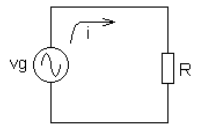
\includegraphics[scale=0.5]{fig1.png}
\end{figure}
La tensión $V_{g}$ tendrá un valor instantáneo que vendrá dado en todo momento por:
$$
V_{g} = V_{0}\sen(2\pi f t)
$$
\chapter{Circuitos transitorios de segundo orden RLC serie}
Un circuito de segundo orden se caracteriza por una ecuación diferencial de segundo orden. Consta de elementos R, L y C.\\
Atención, la rama C es un corto-circuito: de esta manera no se pueden unir las ramas A y B directamente a los bornes de un generador E, se les debe adjuntar una resistencia. Las dos condiciones iniciales son:
\begin{itemize}
\item $i_{l0}$ conserva su valor antes de la puesta en tensión (porque la inductancia se opone a la variación de corriente).
\item $q_{0}$ conserva su valor antes de la puesta en tensión $u_{0} = \frac{q_{0}}{C}$ 
\end{itemize}
La transformación compleja aplicada a las diferentes intensidades proporciona:
$$
I = I_{r} + I_{l} + I_{c}
$$
Los circuitos RLC son generalmente utilizados para realizar filtros de frecuencias, o de transformadores de impedancia. Estos circuitos pueden entonces comportar múltiples inductancias y condensadores: se habla entonces de ``red LC''. Un circuito LC simple es denominado de segundo orden porque su función de transferencia comporta un polinomio de segundo grado en el denominador.
\begin{thebibliography}{99}  %%%este es un contador para el número de bibliografías utilizados.
\addcontentsline{toc}{chapter}{Bibliograf\'{\i}a} %%% Para introducir la bibliografía en el índice.
%\bibitem{Rahman}{Rahman,Aminur y Doe, Hidekazu; ``Ion transfer of tetraalkylammonium cations at an interface between 
%frozen aqueous solution and 1,2-dichloroethane".{\em{Journal of Electroanalytical Chemistry}} {\bfseries 424},159,(1997).}
\bibitem{Gro}{Boylestad, Robert M. ``Introducción al análisis de circuitos''. {\em{Pearson}}}
\bibitem{Gro}{Sadiku, Matthew N. ``Fundamemtos de circuitos eléctricos''. {\em{Mc Graw Hill}}}
%\bibitem{Ding}{Ding, Zhifeng. ``Spectroelectrochemistry and photoelectrochemistry of charge transfer at liquid/liquid
%interfaces". {\em {Tesis, EPFL,}}(1999).}
%\bibitem{AL}{Alonso, Jose M. \em{Técnicas de mecanizado 1}}
%\bibitem{AL}{Alonso, Jose M. ``Técnicas de mecanizado 1". {\em{Paraninfo}} {\bfseries España-Madrid}, 6-20, (2001).}
%\bibitem{Samec2}{Samec Z., Lhotsky A., Jänchenová H., y Marecek, V. ``Interfacial tension and impedance measurements
%of interfaces between two inmiscible electrolyte solutions". {\em{Journal of Electroanalytical Chemistry}} {\bfseries
%43}, 47, (2000).}
%\bibitem{Day}{Day R.A. y Underwood A.L. {\textit{Química Analítica Cuantitativa}},5ºed. Prentice-Hall, México, 1998. 45-48.}
%\bibitem{Keyser}{Farah Abud, Michel. ``Determinación de la vida útil en herramientales de corte endurecido por el proceso de borurización en pasta''. {\em{Instituto tecnológico y de estudios superiores de Monterrey}}}
%\bibitem{Zolotorevski}{Escalona, I. ``Máquinas: herramientas por arranque de viruta.''.{\em{El Cid Editor.}}}
%\bibitem{Lasheras}{Lasheras. ``Tecnología de los Materiales Industriales''.} 
%\bibitem{Dieter}{Dieter. ``Metalurgia mecánica''.}
%\bibitem{Apraiz}{Apraiz, J. ``Tratamiento Térmico de los Aceros''.}
%\bibitem{Smith}{Smith, William F. y Ph.D. Hashemi, Javad ``Ciencia e ingeniería de materiales". {\em{
%Madrid: McGraw-Hill, Interamericana de España.}} 570, (2004).} 
%\bibitem{Callister}{Callister, William D. y Rethwisch, David G. ``Introducción a la ingeniería de los materiales''. %{\em{Barcelona Reverté.}}, 960, (2007).} 
%\bibitem{Askeland}{Askeland, Donald R., Pradeep P. Phulé y Wright, Wendelin J. ``Ciencia e ingeniería de los materiales''.{\em{México, D.F. Internacional Thomson Editores.}} {\textit{$6^{ta}$ edición}}, 1004, (2012).}
%\bibitem{HARDBANDING}{Tabla de conversión de escala de durezas. \begin{verbatim}http://%hardbandingsolutions.com/postle_sp/hardness.php
%\end{verbatim}}
%\bibitem{HE}{Fresadora. \begin{verbatim} http://lizdenbow.blogspot.com/
%\end{verbatim}}
%\bibitem{ASTM}{Normas ASTM.}
%\bibitem{NTP}{Normas NTP.}
\end{thebibliography}
\end{document}